\documentclass{beamer}\usepackage[]{graphicx}\usepackage[]{color}
%% maxwidth is the original width if it is less than linewidth
%% otherwise use linewidth (to make sure the graphics do not exceed the margin)
\makeatletter
\def\maxwidth{ %
  \ifdim\Gin@nat@width>\linewidth
    \linewidth
  \else
    \Gin@nat@width
  \fi
}
\makeatother

\definecolor{fgcolor}{rgb}{1, 0.894, 0.769}
\newcommand{\hlnum}[1]{\textcolor[rgb]{0.824,0.412,0.118}{#1}}%
\newcommand{\hlstr}[1]{\textcolor[rgb]{1,0.894,0.71}{#1}}%
\newcommand{\hlcom}[1]{\textcolor[rgb]{0.824,0.706,0.549}{#1}}%
\newcommand{\hlopt}[1]{\textcolor[rgb]{1,0.894,0.769}{#1}}%
\newcommand{\hlstd}[1]{\textcolor[rgb]{1,0.894,0.769}{#1}}%
\newcommand{\hlkwa}[1]{\textcolor[rgb]{0.941,0.902,0.549}{#1}}%
\newcommand{\hlkwb}[1]{\textcolor[rgb]{0.804,0.776,0.451}{#1}}%
\newcommand{\hlkwc}[1]{\textcolor[rgb]{0.78,0.941,0.545}{#1}}%
\newcommand{\hlkwd}[1]{\textcolor[rgb]{1,0.78,0.769}{#1}}%
\let\hlipl\hlkwb

\usepackage{framed}
\makeatletter
\newenvironment{kframe}{%
 \def\at@end@of@kframe{}%
 \ifinner\ifhmode%
  \def\at@end@of@kframe{\end{minipage}}%
  \begin{minipage}{\columnwidth}%
 \fi\fi%
 \def\FrameCommand##1{\hskip\@totalleftmargin \hskip-\fboxsep
 \colorbox{shadecolor}{##1}\hskip-\fboxsep
     % There is no \\@totalrightmargin, so:
     \hskip-\linewidth \hskip-\@totalleftmargin \hskip\columnwidth}%
 \MakeFramed {\advance\hsize-\width
   \@totalleftmargin\z@ \linewidth\hsize
   \@setminipage}}%
 {\par\unskip\endMakeFramed%
 \at@end@of@kframe}
\makeatother

\definecolor{shadecolor}{rgb}{.97, .97, .97}
\definecolor{messagecolor}{rgb}{0, 0, 0}
\definecolor{warningcolor}{rgb}{1, 0, 1}
\definecolor{errorcolor}{rgb}{1, 0, 0}
\newenvironment{knitrout}{}{} % an empty environment to be redefined in TeX

\usepackage{alltt}
\usepackage{../371g-slides}
% Uncomment these lines to print notes pages
% \pgfpagesuselayout{4 on 1}[letterpaper,border shrink=5mm,landscape]
% \setbeameroption{show only notes}
\title{Introduction to R}
\subtitle{Lecture 2}
\author{STA 371G}
\IfFileExists{upquote.sty}{\usepackage{upquote}}{}
\begin{document}





  \frame{\maketitle}

  %%%%%%% Slides start here %%%%%%%

  \begin{darkframes}



    \begin{frame}{RStudio}
     R is the language, which we access through RStudio (interface).\pause
      \begin{center}
        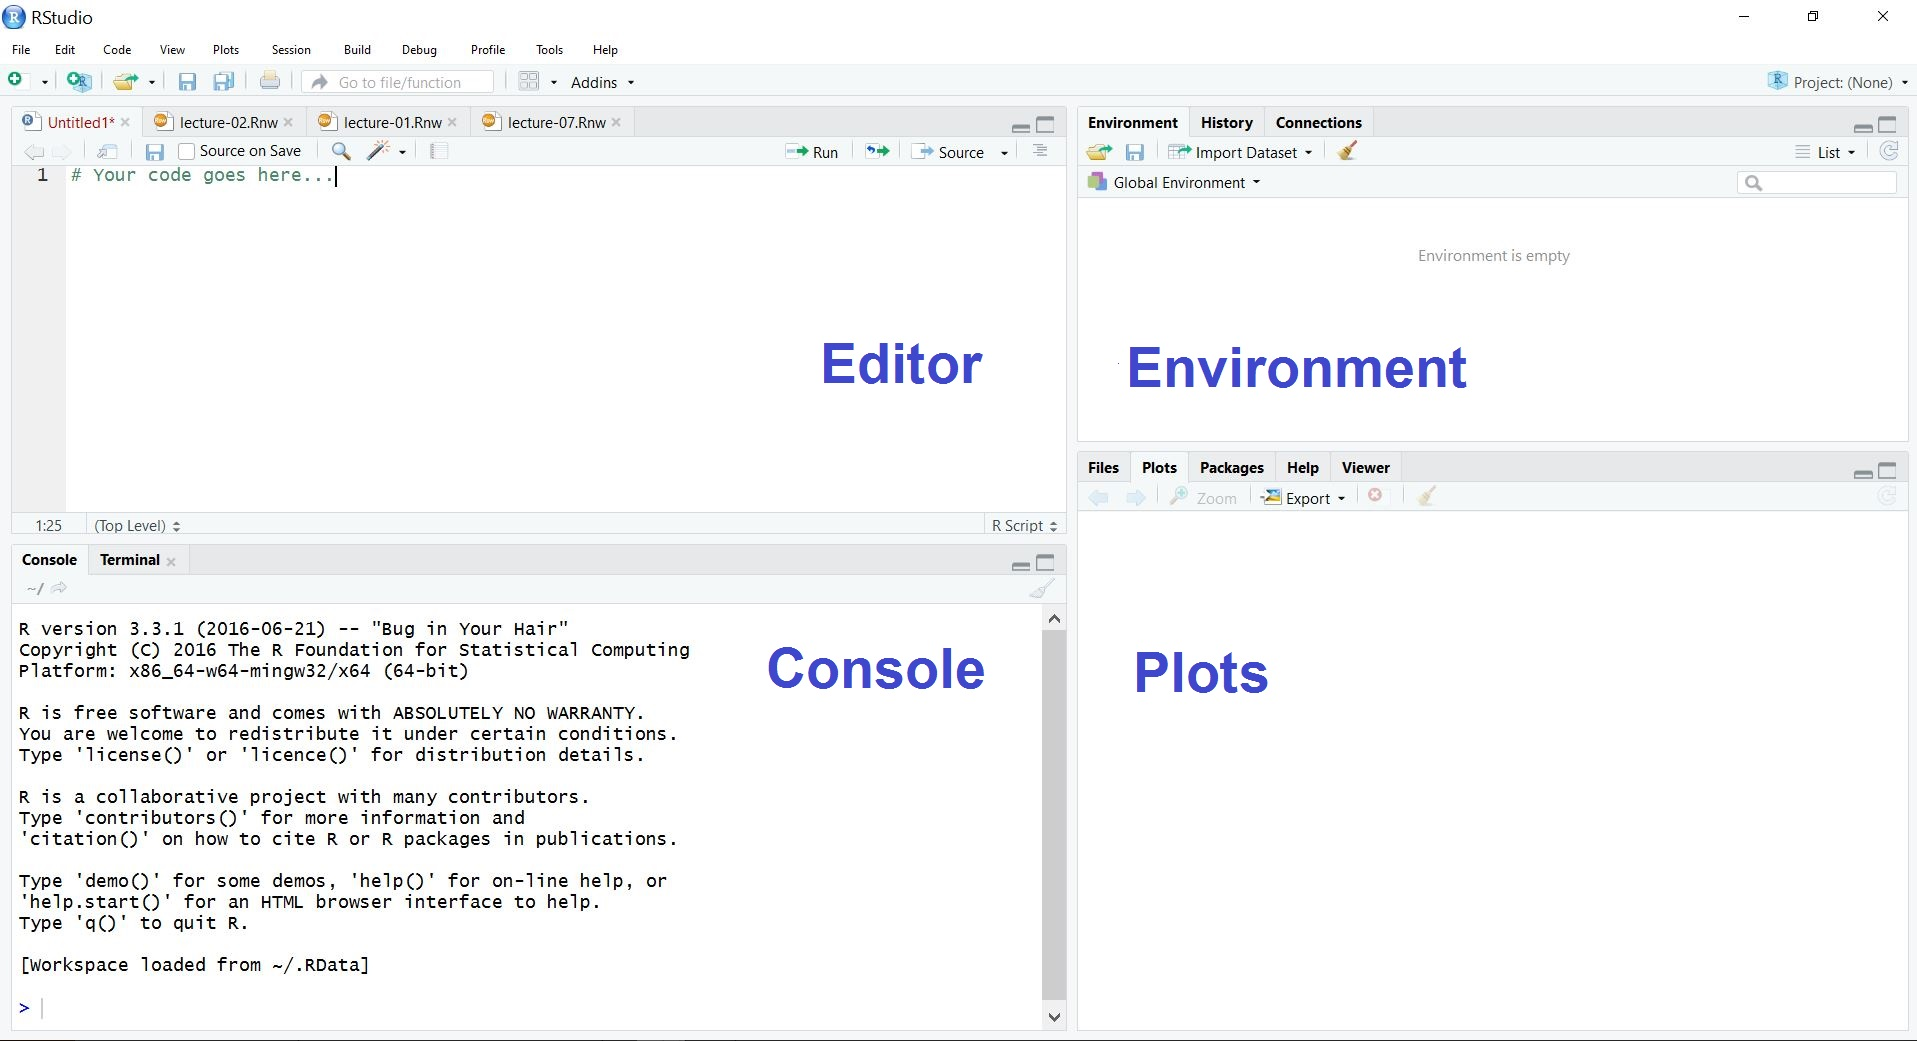
\includegraphics[width=\textwidth]{RStudio}
      \end{center}
    \end{frame}

    \begin{frame}{RStudio}
      \begin{itemize}
        \item \alert{Console:} This is where calculations/code are passed to R and results are observed. \pause
        \item \alert{Editor:} It is not practical to write long calculations/code in console. We write them in the editor, and "Run" to pass to the console. \pause
        \item \alert{Environment:} All data sets/variables we define can be found here. \pause
        \item \alert{Plots:} When we plot things, they will first appear here.
      \end{itemize}
    \end{frame}

    \begin{frame}{Let's get started...}
    Suppose you want to calculate your course grade.

    \begin{table}[!b]
      \begin{tabular}{ccc}
         Assignment & Weight  & Grade \\
        \toprule
          Class participation & 5\%	&	91  \\
          Reading assignments & 5\%	&	95  \\
          Homework    & 15\%	&	 86 \\
          Project     & 15\%	&	 83 \\
          Midterm 1   & 20\%	&	 88 \\
          Midterm 2   & 20\%	&	 84 \\
          Final exam  & 20\%	&	 76 \\
      \end{tabular}
    \end{table}
    \end{frame}


    \begin{frame}[fragile]{Using the console}
      Try this in the console (enter all on one line and press Enter):
\begin{knitrout}
\definecolor{shadecolor}{rgb}{0.137, 0.137, 0.137}\begin{kframe}
\begin{alltt}
\hlnum{0.05}\hlopt{*}\hlnum{91} \hlopt{+} \hlnum{0.05}\hlopt{*}\hlnum{95} \hlopt{+} \hlnum{0.15}\hlopt{*}\hlnum{86} \hlopt{+} \hlnum{0.15}\hlopt{*}\hlnum{83} \hlopt{+}
  \hlnum{0.2}\hlopt{*}\hlnum{88} \hlopt{+} \hlnum{0.2}\hlopt{*}\hlnum{84} \hlopt{+} \hlnum{0.2}\hlopt{*}\hlnum{76}
\end{alltt}
\begin{verbatim}
[1] 84.25
\end{verbatim}
\end{kframe}
\end{knitrout}
    \end{frame}

    \begin{frame}[fragile]{Using the console}
      We can also assign the result of a calculation to a variable.
      Here we'll create a variable called \verb|grade| which will contain
      the result of our calculation:

\begin{knitrout}
\definecolor{shadecolor}{rgb}{0.137, 0.137, 0.137}\begin{kframe}
\begin{alltt}
\hlstd{grade} \hlkwb{<-} \hlnum{0.05}\hlopt{*}\hlnum{91} \hlopt{+} \hlnum{0.05}\hlopt{*}\hlnum{95} \hlopt{+} \hlnum{0.15}\hlopt{*}\hlnum{86} \hlopt{+} \hlnum{0.15}\hlopt{*}\hlnum{83} \hlopt{+}
  \hlnum{0.2}\hlopt{*}\hlnum{88} \hlopt{+} \hlnum{0.2}\hlopt{*}\hlnum{84} \hlopt{+} \hlnum{0.2}\hlopt{*}\hlnum{76}
\end{alltt}
\end{kframe}
\end{knitrout}

      \pause

      Now we can do calculations using that variable. For example,
      what will our grade be if the grades are curved up by 5 points?

\begin{knitrout}
\definecolor{shadecolor}{rgb}{0.137, 0.137, 0.137}\begin{kframe}
\begin{alltt}
\hlstd{grade} \hlopt{+} \hlnum{10}
\end{alltt}
\begin{verbatim}
[1] 94.25
\end{verbatim}
\end{kframe}
\end{knitrout}
    \end{frame}

    \begin{frame}[fragile]{Using the editor}
      In R, an \emph{vector} is just a list of numbers.
      Let's redo the calculation using vectors:

\begin{knitrout}
\definecolor{shadecolor}{rgb}{0.137, 0.137, 0.137}\begin{kframe}
\begin{alltt}
\hlcom{# This is the same calculation, using vectors.}
\hlstd{weights} \hlkwb{<-} \hlkwd{c}\hlstd{(}\hlnum{0.05}\hlstd{,} \hlnum{0.05}\hlstd{,} \hlnum{0.15}\hlstd{,} \hlnum{0.15}\hlstd{,} \hlnum{0.2}\hlstd{,} \hlnum{0.2}\hlstd{,} \hlnum{0.2}\hlstd{)}
\hlstd{grades} \hlkwb{<-} \hlkwd{c}\hlstd{(}\hlnum{91}\hlstd{,} \hlnum{95}\hlstd{,} \hlnum{86}\hlstd{,} \hlnum{83}\hlstd{,} \hlnum{88}\hlstd{,} \hlnum{84}\hlstd{,} \hlnum{76}\hlstd{)}
\hlstd{weighted.grades} \hlkwb{<-} \hlstd{weights} \hlopt{*} \hlstd{grades}
\hlstd{my371} \hlkwb{<-} \hlkwd{sum}\hlstd{(weighted.grades)}
\end{alltt}
\end{kframe}
\end{knitrout}
      The multiplication is ``element-wise,'' meaning that the corresponding elements in each vector are multiplied. \pause

      Then, the \verb|sum| function adds up all the elements in the resulting vector.

      \note{Discuss why it makes sense to vectorize and save in variables. We can, for example, use weights in multiple places.}

    \end{frame}



    \begin{frame}[fragile]{Working with tabular data}
      Many data sets we will work with are in tabular format, saved in ``CSV'' files (CSV = comma-separated values).

      \bigskip\pause

      Let's analyze the passenger data from the Titanic disaster. Load the file by copying and pasting the command from Learning Catalytics, and then type \verb|View(titanic)| to view the data set.

      \bigskip\pause

      This data has five variables:
      \begin{itemize}
        \item \alert{Name}: The name of the passenger
        \item \alert{PClass}: The class of the passenger (1st, 2nd, etc)
        \item \alert{Age}: The age of the passenger, in years
        \item \alert{Sex}: The sex of the passenger
        \item \alert{Survived}: Whether the passenger survived the disaster
      \end{itemize}
    \end{frame}



    \begin{frame}[fragile]{Working with tabular data}
      \verb|$| is used to refer to a particular column in the data, such as \verb|titanic$Name|.   \pause

      \bigskip

      To access to an element in a particular position, e.g., row 1, column 4, use \verb|titanic[1,4]|.


    \end{frame}


    \begin{frame}[fragile]{Exploring Categorical Variables}
      The dataset has both quantitative and categorical data. (What's the difference?)

      \bigskip\pause

      Let's explore the categorical variables through some frequency tables.

      Let's say we want to get a frequency table of the number of passengers by class:

\begin{knitrout}
\definecolor{shadecolor}{rgb}{0.137, 0.137, 0.137}\begin{kframe}
\begin{alltt}
\hlkwd{table}\hlstd{(titanic}\hlopt{$}\hlstd{PClass)}
\end{alltt}
\begin{verbatim}

1st 2nd 3rd 
323 279 711 
\end{verbatim}
\end{kframe}
\end{knitrout}
    \end{frame}


    \begin{frame}[fragile]{Exploring Categorical Variables}
      What is more interesting is a two-way table showing how many people survived in each passenger class. We'll assign the table to a variable for later use!

\begin{knitrout}
\definecolor{shadecolor}{rgb}{0.137, 0.137, 0.137}\begin{kframe}
\begin{alltt}
\hlstd{class_survival} \hlkwb{<-} \hlkwd{table}\hlstd{(titanic}\hlopt{$}\hlstd{Survived, titanic}\hlopt{$}\hlstd{PClass)}
\hlstd{class_survival}
\end{alltt}
\begin{verbatim}
     
      1st 2nd 3rd
  No  130 160 573
  Yes 193 119 138
\end{verbatim}
\end{kframe}
\end{knitrout}
    \end{frame}


    \begin{frame}[fragile]{Exploring Categorical Variables}
      To get a better sense of the data, let's calculate the survival percentage for each passenger class.
\begin{knitrout}
\definecolor{shadecolor}{rgb}{0.137, 0.137, 0.137}\begin{kframe}
\begin{alltt}
  \hlkwd{prop.table}\hlstd{(class_survival,} \hlnum{2}\hlstd{)}
\end{alltt}
\begin{verbatim}
     
            1st       2nd       3rd
  No  0.4024768 0.5734767 0.8059072
  Yes 0.5975232 0.4265233 0.1940928
\end{verbatim}
\end{kframe}
\end{knitrout}
      \pause

      It looks like one's chance of survival highly depended on his/her passenger class!
    \end{frame}



    \begin{frame}[fragile]{Slicing the data}
      One very common operation is slicing the data, i.e., selecting the portion that satisfy certain conditions. \pause

      \bigskip
      For example, we can select the rows that belong to female passenger data.
\begin{knitrout}
\definecolor{shadecolor}{rgb}{0.137, 0.137, 0.137}\begin{kframe}
\begin{alltt}
\hlstd{female.passengers} \hlkwb{<-} \hlkwd{subset}\hlstd{(titanic, Sex} \hlopt{==} \hlstr{"female"}\hlstd{)}
\end{alltt}
\end{kframe}
\end{knitrout}
      \pause

      This means: in the titanic dataset, select rows where \verb|Sex| is \verb|female| and save the resulting table to the \verb|female.passengers| variable.

    \end{frame}




    \begin{frame}[fragile]{Slicing the data}
      We can create more complex conditions -- what do you think this does?

\begin{knitrout}
\definecolor{shadecolor}{rgb}{0.137, 0.137, 0.137}\begin{kframe}
\begin{alltt}
\hlstd{my.data} \hlkwb{<-} \hlkwd{subset}\hlstd{(titanic, Sex} \hlopt{==} \hlstr{"female"} \hlopt{&}
                           \hlstd{PClass} \hlopt{==} \hlstr{"1st"}\hlstd{)}
\end{alltt}
\end{kframe}
\end{knitrout}

      \pause

      We can use the \verb|nrow| function to count the \underline{n}umber of \underline{row}s in a dataset:

\begin{knitrout}
\definecolor{shadecolor}{rgb}{0.137, 0.137, 0.137}\begin{kframe}
\begin{alltt}
\hlkwd{nrow}\hlstd{(my.data)}
\end{alltt}
\begin{verbatim}
[1] 143
\end{verbatim}
\end{kframe}
\end{knitrout}

      There were 143 women in first class on the Titanic!
    \end{frame}



    %
    % \begin{frame}[fragile]{Cleaning the data}
    %   \fontsize{10}{10}\selectfont
    %   If you want to analyze the "Age" data, you will realize rows with "NA", meaning Not Available. \pause
    %
    %   \bigskip
    %   Let's select rows where we have age data available.
    %
    %   <<>>=
    %     titanic_age <- titanic[!is.na(titanic$Age),]
    %   @
    %   \pause
    %   This selects rows where the Age value is not "NA".
    %
    % \end{frame}



    \begin{frame}[fragile]{Exploring quantitative data}
      Let's look into age distribution of the passengers.

\begin{knitrout}
\definecolor{shadecolor}{rgb}{0.137, 0.137, 0.137}\begin{kframe}
\begin{alltt}
\hlkwd{hist}\hlstd{(titanic}\hlopt{$}\hlstd{Age,} \hlkwc{col}\hlstd{=}\hlstr{"green"}\hlstd{,}
     \hlkwc{xlab}\hlstd{=}\hlstr{"Passenger age"}\hlstd{,} \hlkwc{main}\hlstd{=}\hlstr{""}\hlstd{)}
\end{alltt}
\end{kframe}
\input{/tmp/figures/unnamed-chunk-13-1.tikz}

\end{knitrout}
    \end{frame}


    \begin{frame}[fragile]{Exploring quantitative data}
      We can look at the relationship between a quantitative variable and a categorical one by generating side-by-side boxplots to compare the distribution of the quantiative variable for each value of the categorical variable:

      \pause

\begin{knitrout}
\definecolor{shadecolor}{rgb}{0.137, 0.137, 0.137}\begin{kframe}
\begin{alltt}
\hlkwd{boxplot}\hlstd{(Age} \hlopt{~} \hlstd{PClass,} \hlkwc{data}\hlstd{=titanic,} \hlkwc{col}\hlstd{=}\hlstr{"green"}\hlstd{,} \hlkwc{main}\hlstd{=}\hlstr{""}\hlstd{)}
\end{alltt}
\end{kframe}
\input{/tmp/figures/unnamed-chunk-14-1.tikz}

\end{knitrout}

      What can we conclude about the relationship between age and class?
    \end{frame}
  \end{darkframes}

\end{document}
